\section{Events}
	\subsubsection{Qualifying competitions}
		\begin{enumerate}
			\item Sochi. 21-23.11.2014. The first experience of team in the competition. At these competition our squad for the first time felt the spirit of competition FCS and noble professionalism. Were getting work experience all day and all night. Began to make acquaintance among the teams simultaneously providing all possible aide.  Plan and organization were very nice. The most memorable was familiarity with the American team "Stuy fission 310", which is now supported by the connection. As a result, gagnered a quota on the regional finals.
			\begin{figure}[H]
				\center{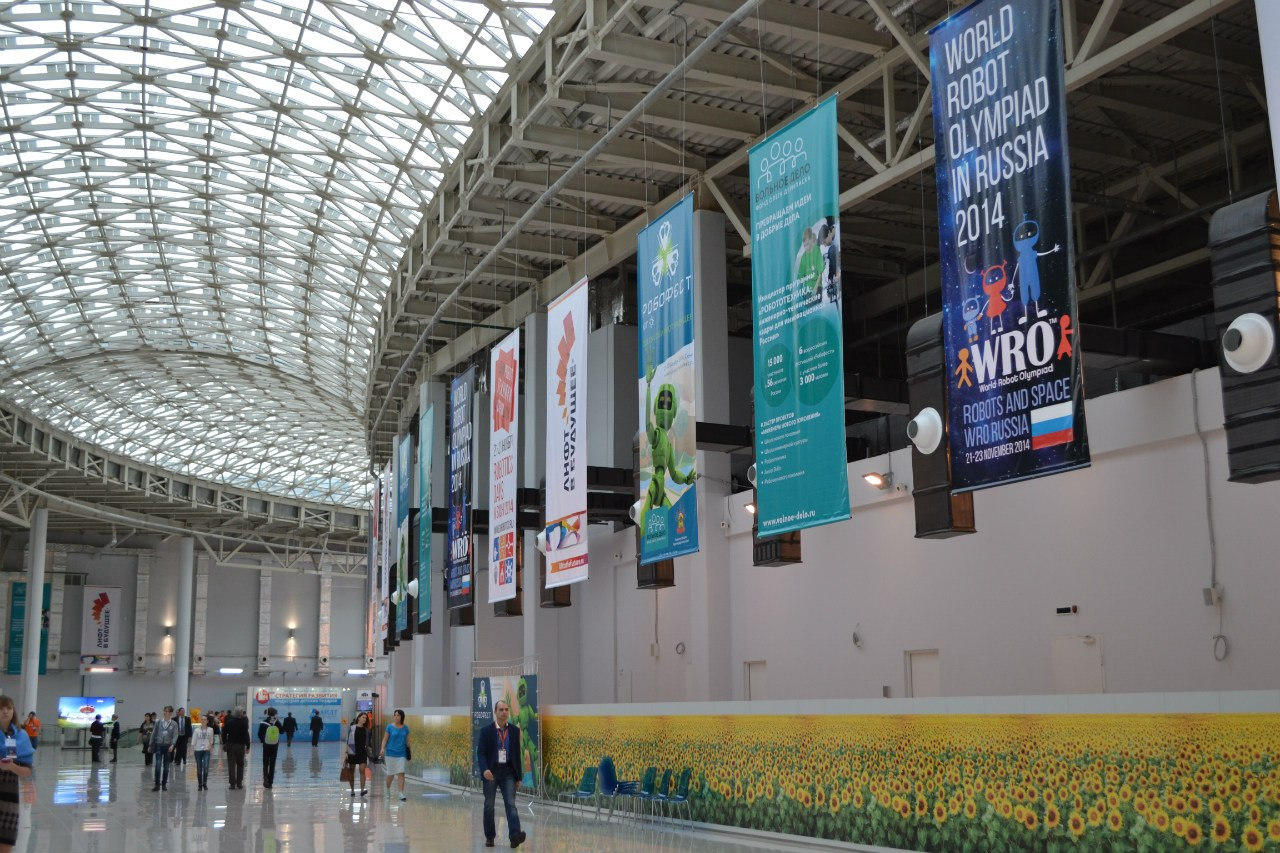
\includegraphics[scale=0.25]{days/Events/images/6}}
			\end{figure}
			\item Ryazan. 13-14.12.2014. In cutting our first priority train on a real field. These competition was enough small and quiet. All teams abundantly communicated and shared ideas. All people feel comfortable there. Team helped to organize example - to assemble and disassemble the field. As a result Participants of the alliance winner. 
			\begin{figure}[H]
				\center{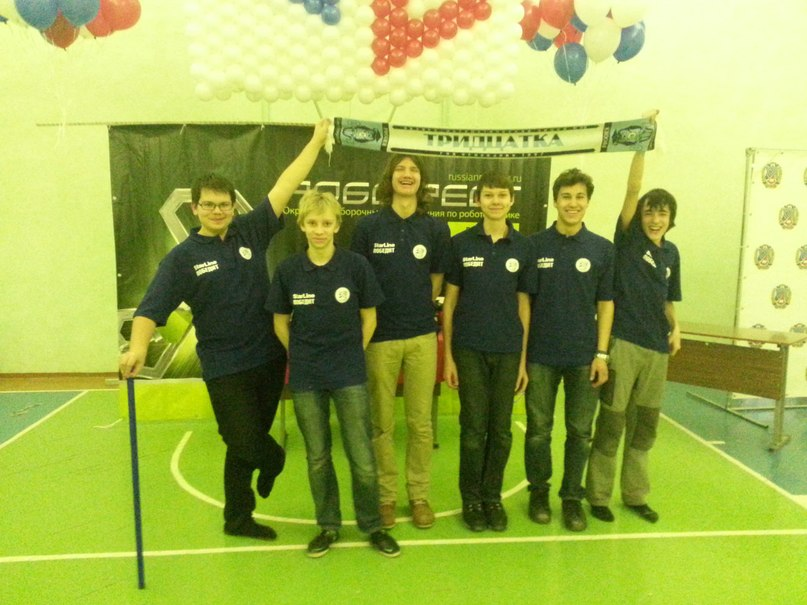
\includegraphics[scale=0.4]{days/Events/images/1}}
	     	\end{figure}	
			\item Perm. 27-29.01.2015. Dress rehearsal before the regional final. It was great organized event where we were able to practice all aspects of the competition. Including such important skills as the choice of Composes alliances finale. Also we strongly helped to organized technical part. As a result, the alliance of winners as well as first place in the general classification.
			\begin{figure}[H]
				\center{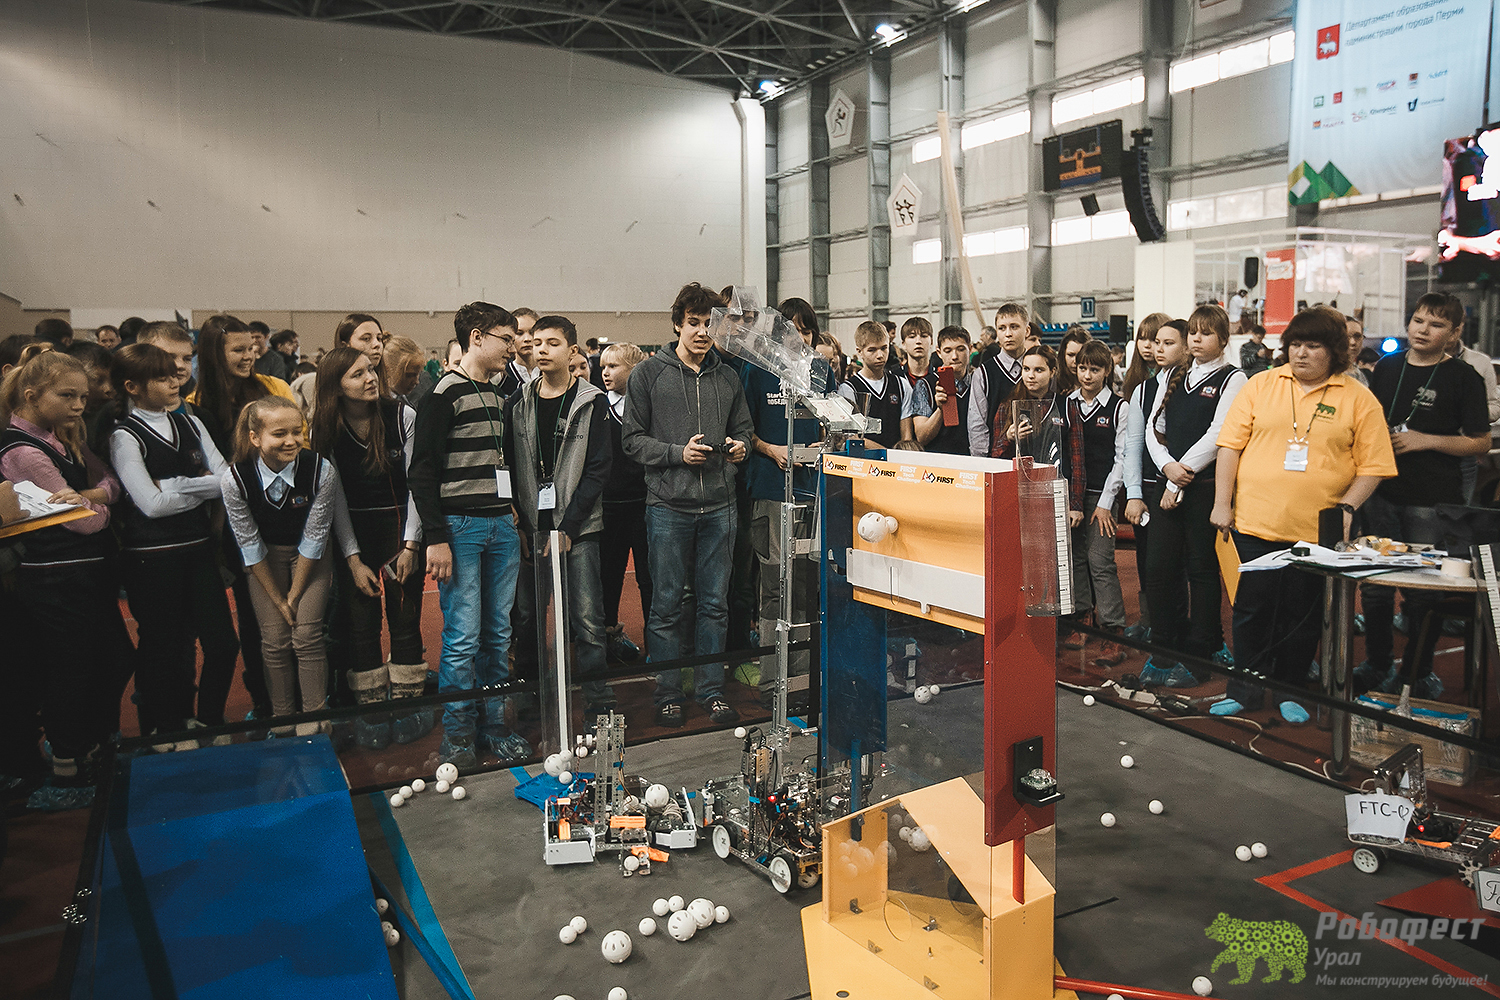
\includegraphics[scale=0.22]{days/Events/images/3}}\\
	     	\end{figure}
		\end{enumerate}  
	\subsubsection{Regional final. 11-13.02.2015}	
		The event, to which the team was preparing for six months, approaching the competition with fully finished. At competitions communicated with all teams, that were there, discussing strategy and offering their help. During the competition, was conducted statistics on all the teams that helped in choosing allies in the final. Also, there was an action plan with many team. In the final, having received a quota on the choice of allies, were chosen team with the most stable results, and the rate was plased at interaction of robots. As a result, the alliance of winners as well as first place in the general classification, and the quota to World Championship.
		\begin{figure}[H]
			\center{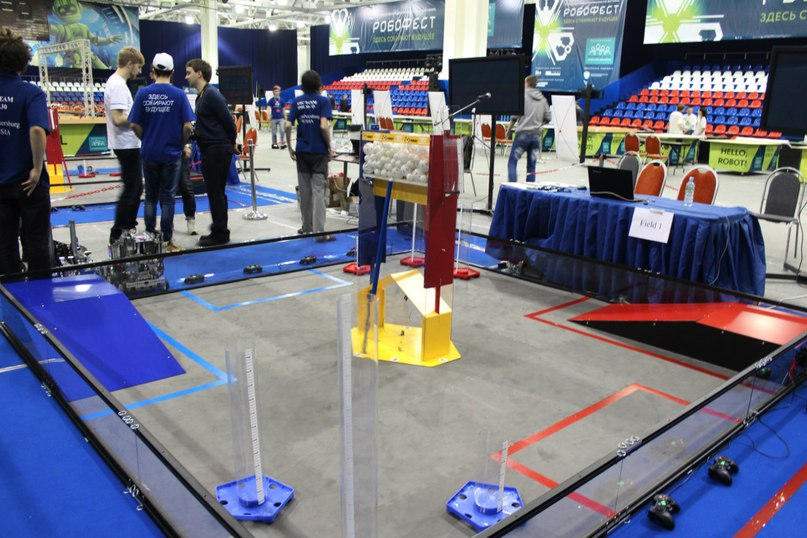
\includegraphics[scale=0.45]{days/Events/images/2}}\\
		\end{figure}
	\newpage			
	\subsubsection{CRDI RTC. 24.11.2014}
	Large Russian Institute of Robotics and Technical Cybernetics. The team was organized hike in institute and we can see the real processes develop detailed design of robotics. We saw several Projects summary at different stages of development - from drawing to finished models, as well as ready-made commercial products. From there we learned some ideas, how to organize. Internet adress: "http://www.rtc.ru".
	\begin{figure}[H]	
		\center{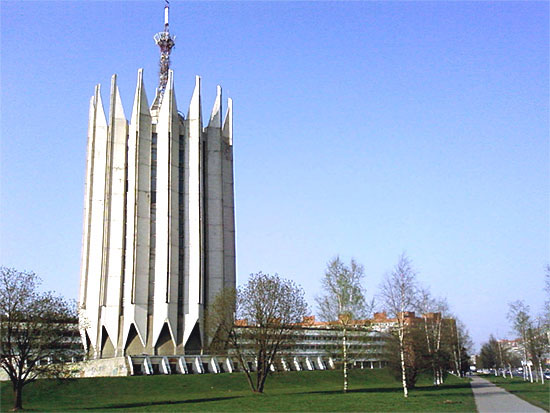
\includegraphics[scale=0.5]{days/Events/images/5}}\\
	\end{figure}
	\subsubsection{PML 30 landfill. 08.02.2015}	
	PML 30 landfill competitions are carried out by our organization. Their main core misrepresented participant receives a task and parts for it's decision merely on the competition, compliance with the maximum being equal. Also, demonstrated the FTC involving the participation.
	\begin{figure}[H]
		\center{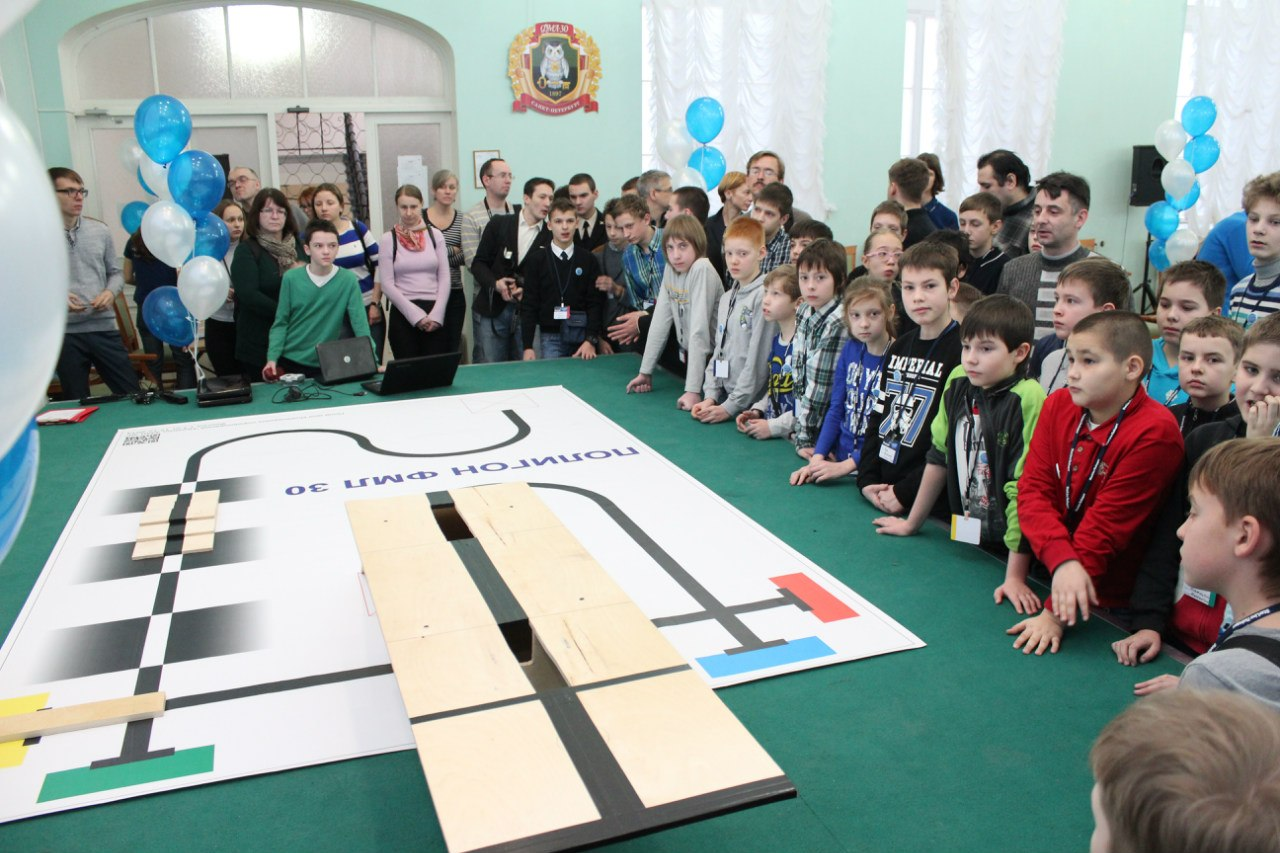
\includegraphics[scale=0.25]{days/Events/images/7}}\\
    \end{figure}
    \subsubsection{GeoScan. 10.03.2015}
    Russian company produces and sells unmanned aerial photography systems. They have clearly shown how the design office, as the allocation of responsibilities and tasks. How is the internal interaction. Also, they have shown the whole production line. Internet adress: "http://geoscan.aero/".
    \begin{figure}[H]
    	\center{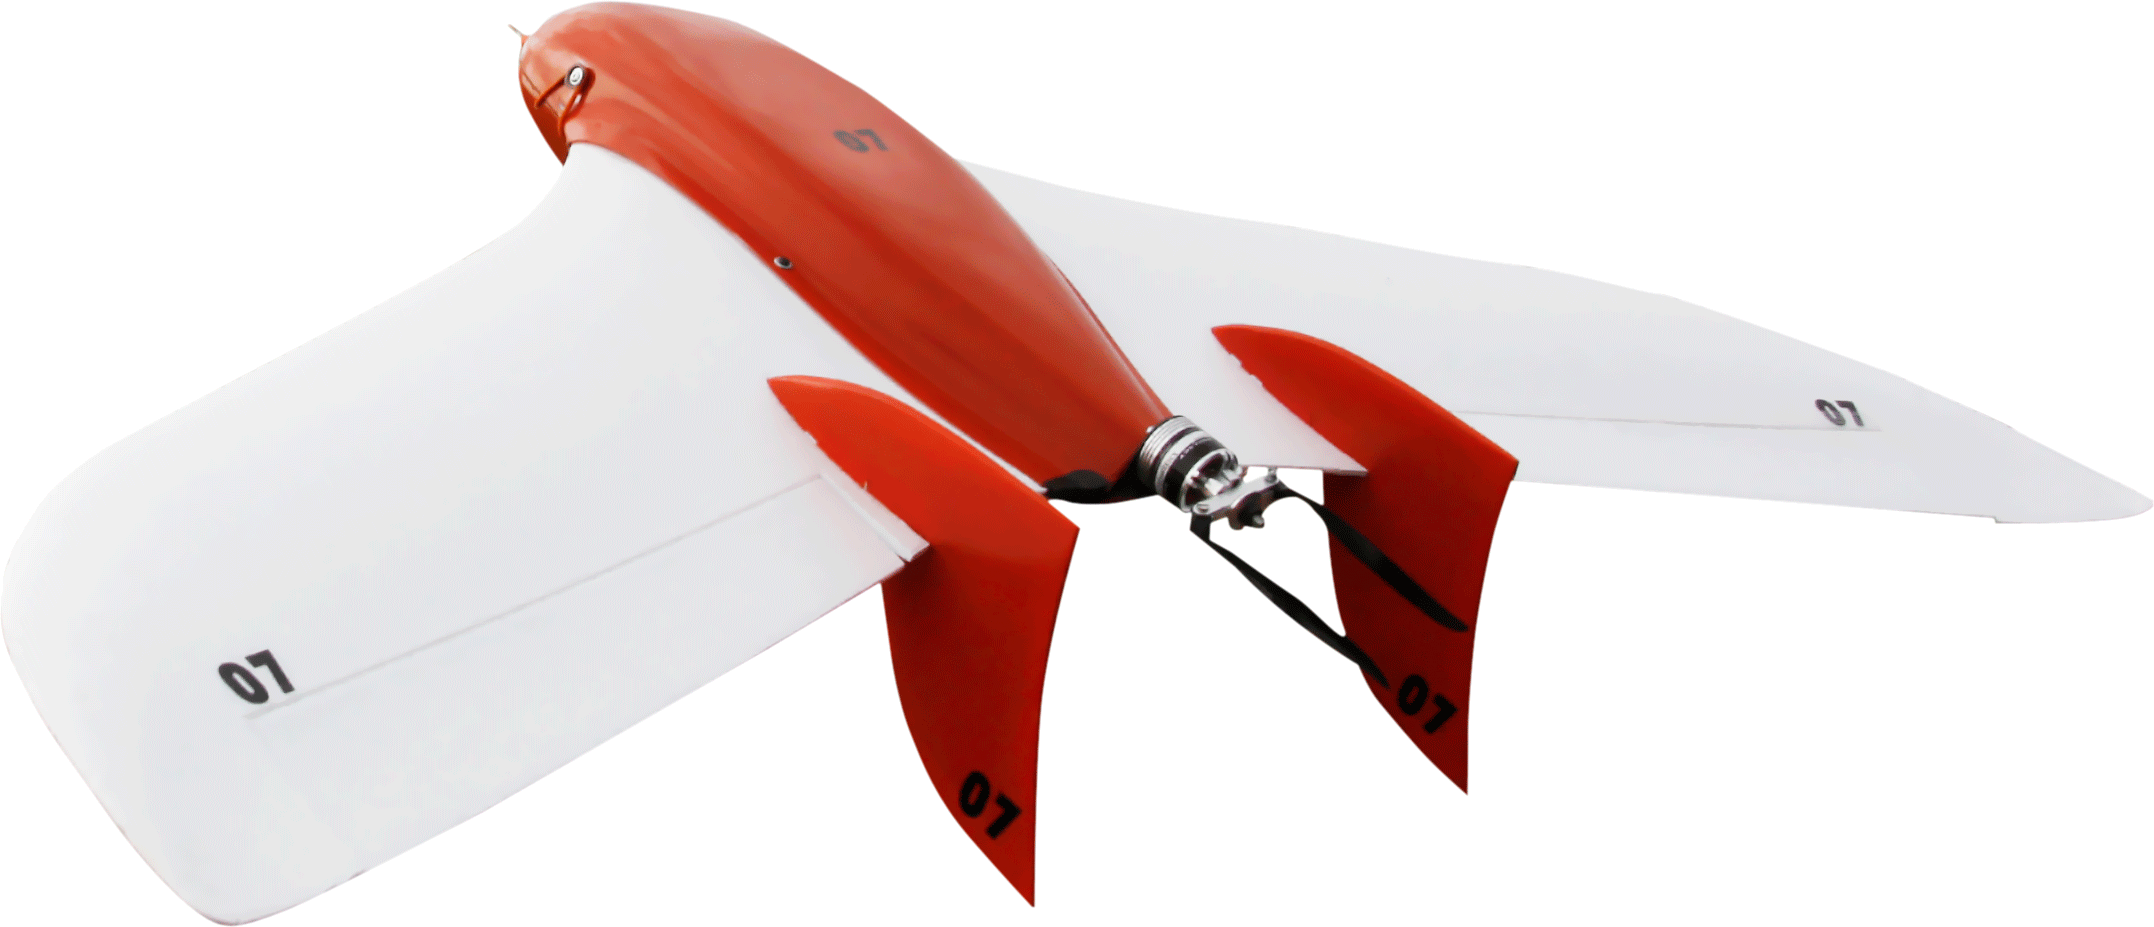
\includegraphics[scale=0.2]{days/Events/images/4}}\\	
    \end{figure}
	\subsubsection{PTC live Tech Forum. 24.03.2015}
	 The team was invited to participate in PTC Live Tech Forum. We will present the successfull path of 3D model creation in Creo Parametric, tell about important tips and show how CAD modelling helped us to build the robot.
	
	\subsubsection{Summer camp on Robotics}
	In the camp in 2015, team members will conduct a robotics engineering course based on constructor TETRIX, attracting more people to the FTC.
	
	\fillpage
		
		
		
		
		
		
		
		
		
